\chapter{Panorama de l'apprentissage artificiel}

Cette partie est destinée à présenter les notions incontournables de l'apprentissage artificiel, sans se prétendre exhaustive ni très détaillée. On y traite de la régression, de la classification, de l'apprentissage supervisé et non supervisé, et enfin des neurones artificiels. Ce panorama est construit par niveau croissant de difficulté des notions, et chaque section fait appel aux précédentes.

\section{Régression \textit{versus} classification}
\subsection{Régression}

La \emph{régression} se caractérise par deux aspects : les entrées de la méthode sont des valeurs numériques continues et la sortie est une autre variable continue. L'idée est contenue dans le nom, c'est-à-dire qu'à partir des diverses mesures effectuées, on tente de tout résumer pour en déduire une autre valeur\footnote{Ici, les variables continues n'évoluent pas dans un ensemble continu de valeurs tels que décrits par la théorie des ensembles. En fait, on pourrait se contenter de savoir s'il existe une relation d'ordre entre les valeurs, et si ces dernières sont nombreuses, pour conclure que la variable est continue.}.

Un exemple typique est celui d'une maison dont on cherche à estimer le prix. Si l'on considère uniquement sa surface habitable, on pourra éventuellement en prédire le prix, mais il faut s'attendre à se tromper assez lourdement. En revanche, si l'on prend en considération l'âge,la durée depuis la mise en vente, l'efficacité thermique, le prix moyen des maisons environnantes, on peut affiner notre estimation. Pour prédire un tel prix, il suffit de construire un modèle, de le tester sur un grand jeu de données réelles puis de l'ajuster. Une difficulté est que, selon le modèle qu'on prend, ses paramètres ne sont pas forcément uniques. On peut donc être amené à tester un grand nombre de paramètres mais aussi un grand nombre de modèles si l'on souhaite ouvrir une agence immobilière et fixer des prix.

Le modèle de régression le plus connu est la \emph{régression linéaire}. Ses hypothèses sont simples : la variable prédite est une combinaison linéaire des variables d'entrées. Dans le cas de notre exemple, si nous appelons \(\hat y\) le prix de la maison, \(x_i\) les variables d'entrée et \(\alpha_i\) les paramètres du modèle, alors la prédiction s'écrit :
\[\hat{y} = \alpha_0 + \sum_{i = 1}^{i = n}{\alpha_i x_i}\]
ou encore 
\begin{equation} \label{eq:reg_lin}
\hat{y} = \langle \boldsymbol{\alpha}, \boldsymbol{x} \rangle
\end{equation}
en notation vectorielle, où : \(\boldsymbol{\alpha}\) est le vecteur des \(n + 1\) paramètres; \(\boldsymbol{x}\) est le vecteur des paramètres, de dimension \(n + 1\), dont le premier vaut 1;  \(\langle, \rangle\), représente le produit scalaire.

Ainsi, avec un seul paramètre, par exemple la surface habitable, l'évolution du prix pourrait ressembler à la figure \ref{fig:reg_lin} où chaque point représente une maison dont on a mesuré la surface habitable et consulté le prix de vente.

\begin{figure}
\centering
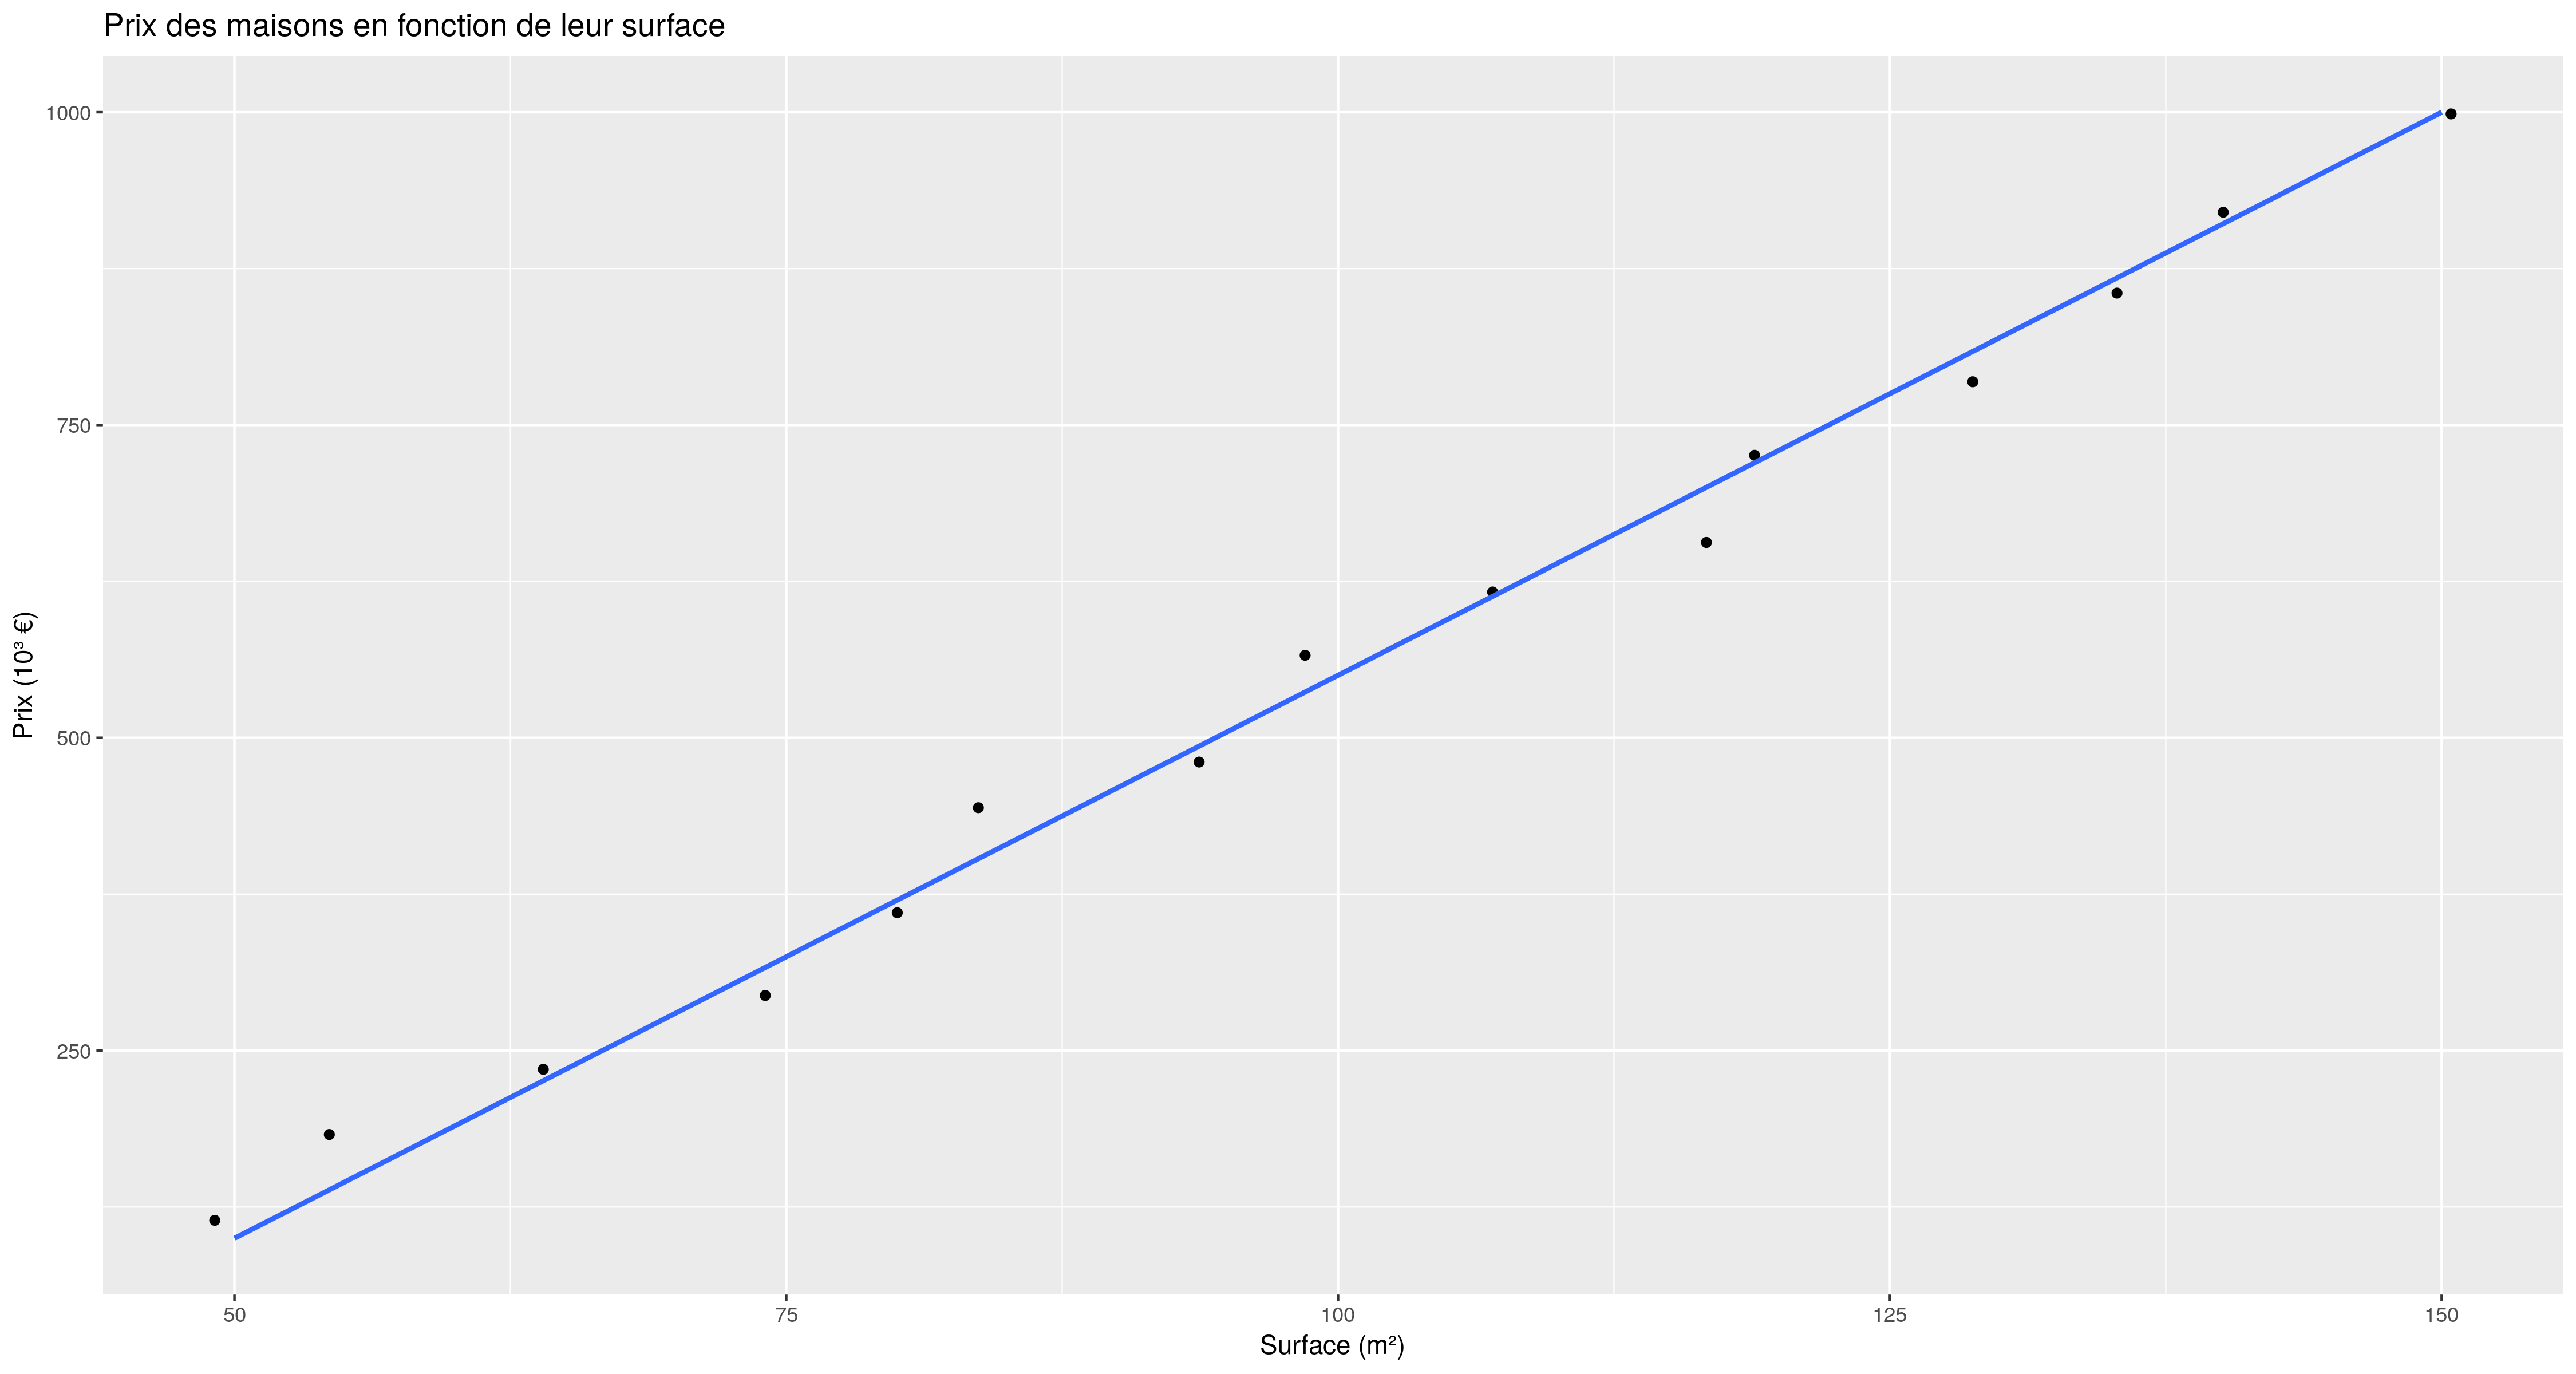
\includegraphics[width=\textwidth]{img/reg_lin.png}
\caption{Régression linéaire sur la surface habitable}
\label{fig:reg_lin}
\end{figure}

Ce modèle est souvent privilégié du fait de la simplicité de sa mise en œuvre. Bien sûr, on peut imaginer des modèles non linéaires, dans lesquels \(\hat y\) est une fonction non linéaire des \(x_i\). Quelle que soit la régression choisie, il existe une méthode suffisamment générale pour calculer une approximation des meilleurs paramètres du modèle, nous la verrons plus loin.

Le choix du modèle se fait par souci de \emph{généralisation}, c'est-à-dire qu'un modèle sera privilégié s'il permet de prédire des prix réalistes au-delà du seul jeu de données sur lequel il a été construit. Là encore, nous verrons plus loin comment parvenir à un modèle satisfaisant dans le cas général. 

Enfin, il est possible de faire une régression sur des variables catégorielles, mais il faut au préalable les "numériser". Cette méthode est appelée "analyse factorielle des correspondances", mais les détails importent peu ici.

Voyons maintenant un autre pilier sur lequel peut s'appuyer un algorithme d'apprentissage pour fonctionner.

\subsection{Classification} 
Contrairement à la régression, la \emph{classification} (\emph{clustering} en anglais) prédit la valeur d'une variable discrète, appelée \emph{classe}, à partir d'entrées continues ou discrètes.

Pour reprendre l'exemple précédent, il pourrait s'agir de prédire si la maison serait éligible au classement des monuments historiques. Dans le premier cas on parle de "classification binaire". Si plus de 3 valeurs sont possibles, on parle de "classification multiple" ou "multiclasses". Parfois, il arrive que des classes ne soient pas mutuellement exclusives, mais nous ne nous en préoccuperons pas ici.

Les modèles de classification sont nombreux et très divers. Ceci est dû au fait que les problèmes auxquels répondent les algorithmes de classification sont eux-mêmes très divers. Pour les modèles, on citera donc pêle-mêle les arbres de décision (et leur amélioration que sont les forêts aléatoires), les \(k\)-plus proches voisins,  les \(k\)-moyennes, ou encore la classification hiérarchique. Deux illustrations par la figure \ref{fig:clusterings}.

\begin{figure}
    \centering
    \begin{subfigure}[b]{0.45\textwidth}
        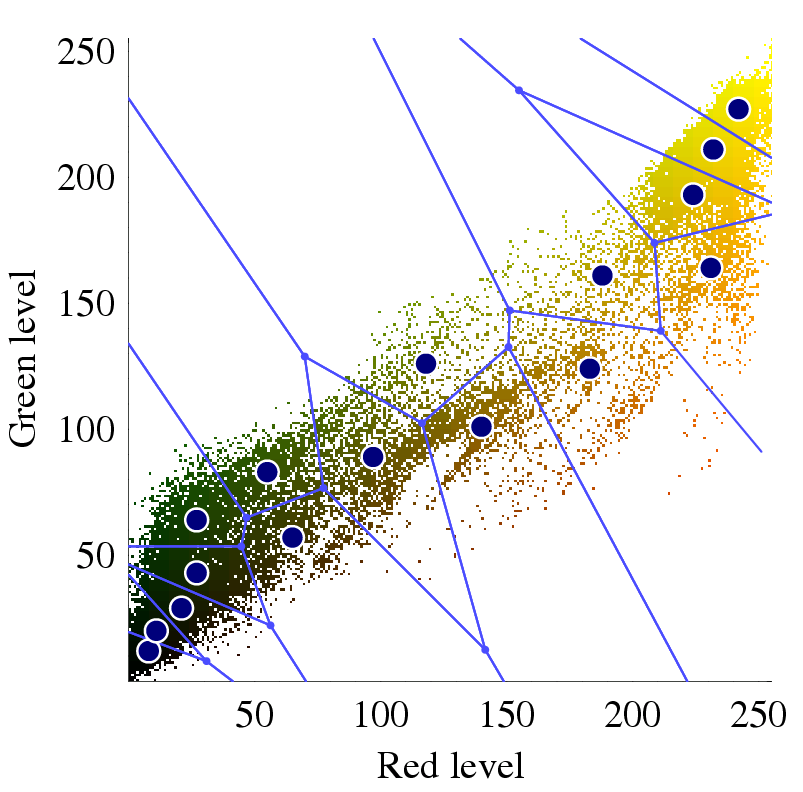
\includegraphics[width=\textwidth]{img/kmeans_voronoi.png}
        \caption{Partitionnement par les \(k\)-moyennes}
    \end{subfigure}
    \begin{subfigure}[b]{0.45\textwidth}
        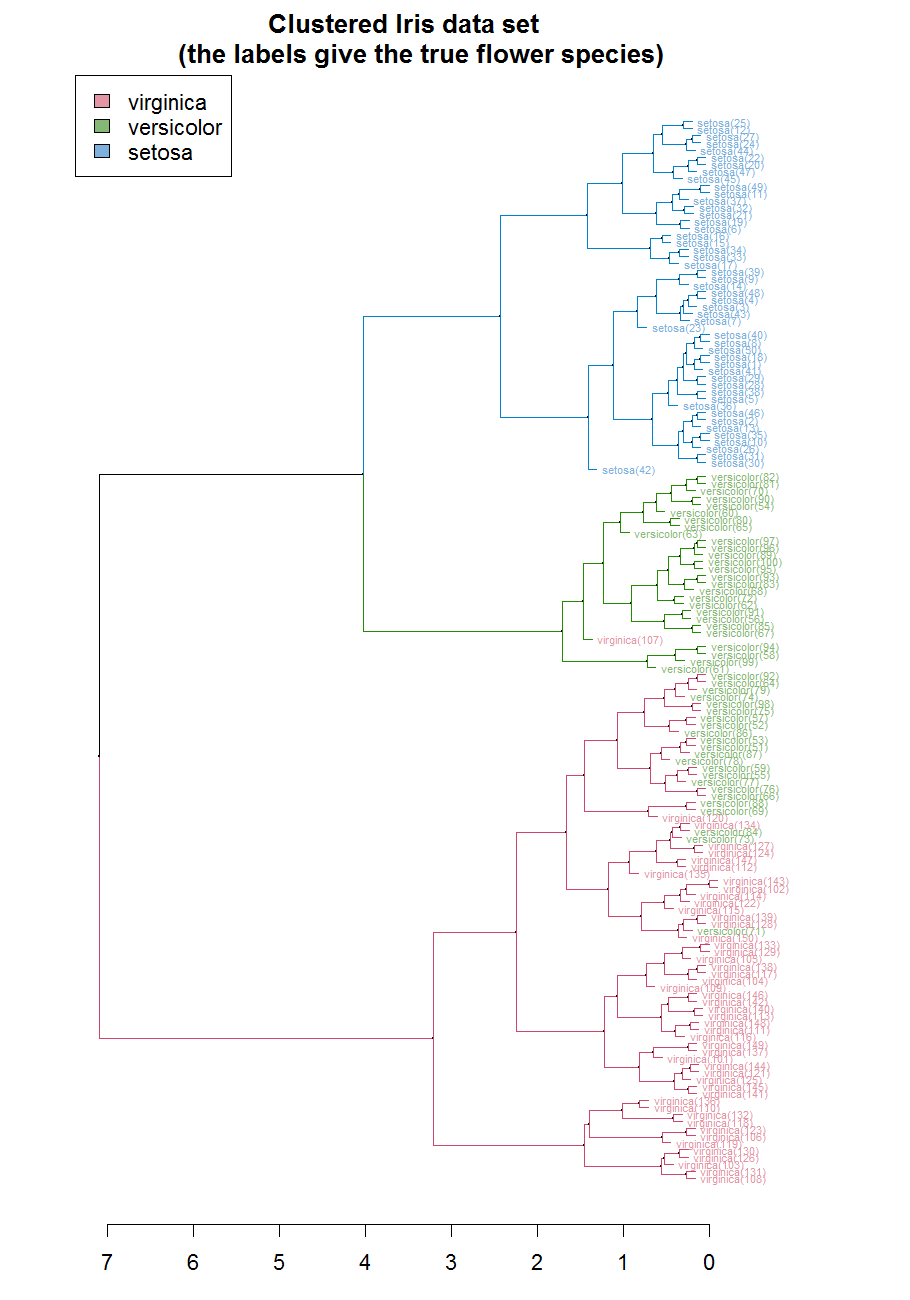
\includegraphics[width=\textwidth]{img/iris_dendrogram.png}
        \caption{Classification ascendante hiérarchique}
    \end{subfigure}
    \caption{Différentes classifications}\label{fig:clusterings}
\end{figure}

Le choix entre ces modèles se fait souvent en fonction de la dimension du problème, mais aussi de la répartition des données dans l'espace des variables. Typiquement, si les données peuvent être séparées par une droite, un plan, ou un hyperplan, alors on se contentera d'un classifieur linéaire adapté à la dimension. Mais il arrive bien souvent que les données ne sont pas séparables linéairement, alors on doit pousser l'analyse plus loin, comme leur appliquer des transformations non linéaires ou les traiter avec des réseaux de neurones.


\subsection*{Conclusion}
Nous avons vu que l'apprentissage artificiel se réduisait à résoudre un problème de type régression, calcul d'une valeur continue, ou bien classification, calcul d'une valeur discrète. Il s'avère que certaines techniques de régression permettent aussi de faire de la classification, typiquement en calculant une probabilité qu'on arrondit ensuite au nombre entier le plus proche (0 ou 1). C'est le cas de la régression ridge par exemple. Nous n'en donnerons pas les détails ici.

Abordons maintenant une autre dichotomie classique du domaine de l'apprentissage.

\section{Apprentissage supervisé \textit{versus} non supervisé}
\subsection{Supervisé}
L'\emph{apprentissage supervisé} consiste simplement à entraîner l'algorithme avec des exemples. On lui soumet un ensemble de données dont on donne le label ou la valeur qu'il devrait prédire et on ajuste les paramètres du modèle pour "coller" à ces exemples. Ainsi, on donnerait 500 instances de maisons et de leurs caractéristiques, ainsi que leur prix (pour la régression) ou le label "bâtiment classé"/"maison ordinaire" (pour la classification).

Plus précisément, on commencera par définir une \emph{fonction de coût} (\emph{loss function} en anglais) dépendant de la réponse attendue et de la réponse réellement produite par le modèle; il s'agit en fait d'une mesure de la performance du modèle sur les données d'entraînement. Pour une régression linéaire, on choisit très souvent la fonction racine de l'erreur quadratique moyenne \(\sqrt{\frac{1}{m}\sum_1^m(\hat y_i - y_i)^2}\), mais d'autres sont possibles. Le but de l'algorithme sera alors de trouver les paramètres du modèle qui minimisent la fonction de coût. Dans le cas particulier d'une régression linéaire, il existe une forme close pour calculer ces paramètres optimaux (lorsque la fonction de coût est la racine de l'erreur quadratique moyenne). Mais dans le cas général, nous ne connaissons pas de formule. Pour trouver les paramètres induisant une bonne performance sur le jeu d'entraînement, on utilise une heuristique (voir la section \ref{subseq:desc_grad}).

Une fois l'algorithme entraîné, donc une fois les paramètres du modèle fixés, on peut lui soumettre des données de test pour voir s'il est capable de généraliser et jusqu'à quel point. Si ces données sont annotées comme lors de la phase d'entraînement, on pourra évaluer le pouvoir de généralisation de l'algorithme, à nouveau grâce à la fonction de perte. Si on n'annote pas ces données de test, on aura simplement une vague idée du comportement sous-jacent de l'algorithme\footnote{Ces dernières années, la classification de photos et d'images a connu un essor impressionnant grâce à des architectures complexes de réseaux de neurones, et les performances des algorithmes frôlent le sans-faute très souvent. Il existe cependant une manière particulière de tester les algorithmes, volontairement malicieuse : il s'agit de "l'attaque à 1 pixel" (ou sa généralisation, "construction adversariale"). Il s'agit de modifier un unique pixel, bien choisi, d'une image, de sorte que l'algorithme se trompe dans sa prédiction. Sur une image de 32x32 pixels 3 canaux, cela représente donc une perturbation de moins de 0.01\% des données. De manière similaire, on peut modifier de multiples pixels d'une image, sans que ce soit visible à l'œil nu et de sorte à tromper l'algorithme. Dans ces deux cas, la question de la sécurité offerte par ces algorithmes est centrale, et de nombreuses recherches sont en cours.}.

\subsection{Non supervisé}
La caractéristique commune à toutes les méthodes d'\emph{apprentissage non supervisé} est l'absence de phase d'entraînement par l'exemple, contrairement à l'apprentissage supervisé. La motivation première pour employer de telles techniques est de mettre en lumière des structures sous-jacentes des données, ce qui s'apparente donc à des statistiques exploratoires multidimensionnelles. Diverses méthodes peuvent s'apparenter à de l'apprentissage non supervisé, comme la réduction de dimmensionnalité (notamment par l'analyse en composantes principales) ou la détection d'anomalies (avec les réseaux bayésiens par exemple). Ici encore, ces méthodes peuvent être réduites à une classification (garder ou non une variable, considérer une observation comme normale ou anormale), ou à une régression (distance moyenne entre deux points de l'espace des variables); ou encore, une régression dont on déduit une classe. 

Malheureusement, l'apprentissage non supervisé le plus général dépasse largement le cadre de ce projet. Continuons donc sur les tant plébiscités neurones artificiels.


\section{Notion de neurone artificiel}
Les sciences s'inspirent parfois de caractères trouvés dans la nature et essaye de les imiter. Mais l'imitation ne réussit pas toujours aussi bien que l'original. Si l'on s'était profondément inspiré des oiseaux pour voler, nos avions battraient des ailes. Or, laisser de côté le biomimétisme a permis le développement des turboréacteurs nous permettant de nous déplacer quasiment à la vitesse du son lors d'un voyage de routine.

Pour les neurones, l'histoire est sensiblement la même. Les neurones biologiques sont des cellules fonctionnant en réseau et dont un des rôles est de transmettre des impulsions électriques. L'interconnexion entre ces neurones se fait par voie chimique, et leur agencement change au cours de la vie.

\subsection{Unité Linéaire à Seuil}
L'Unité Linéaire à Seuil (ULS, ou Linear Threshold Unit, LTU en anglais) est un composant numérique qui à plusieurs entrées pondérées associe une sortie binaire.

\begin{figure}
\centering
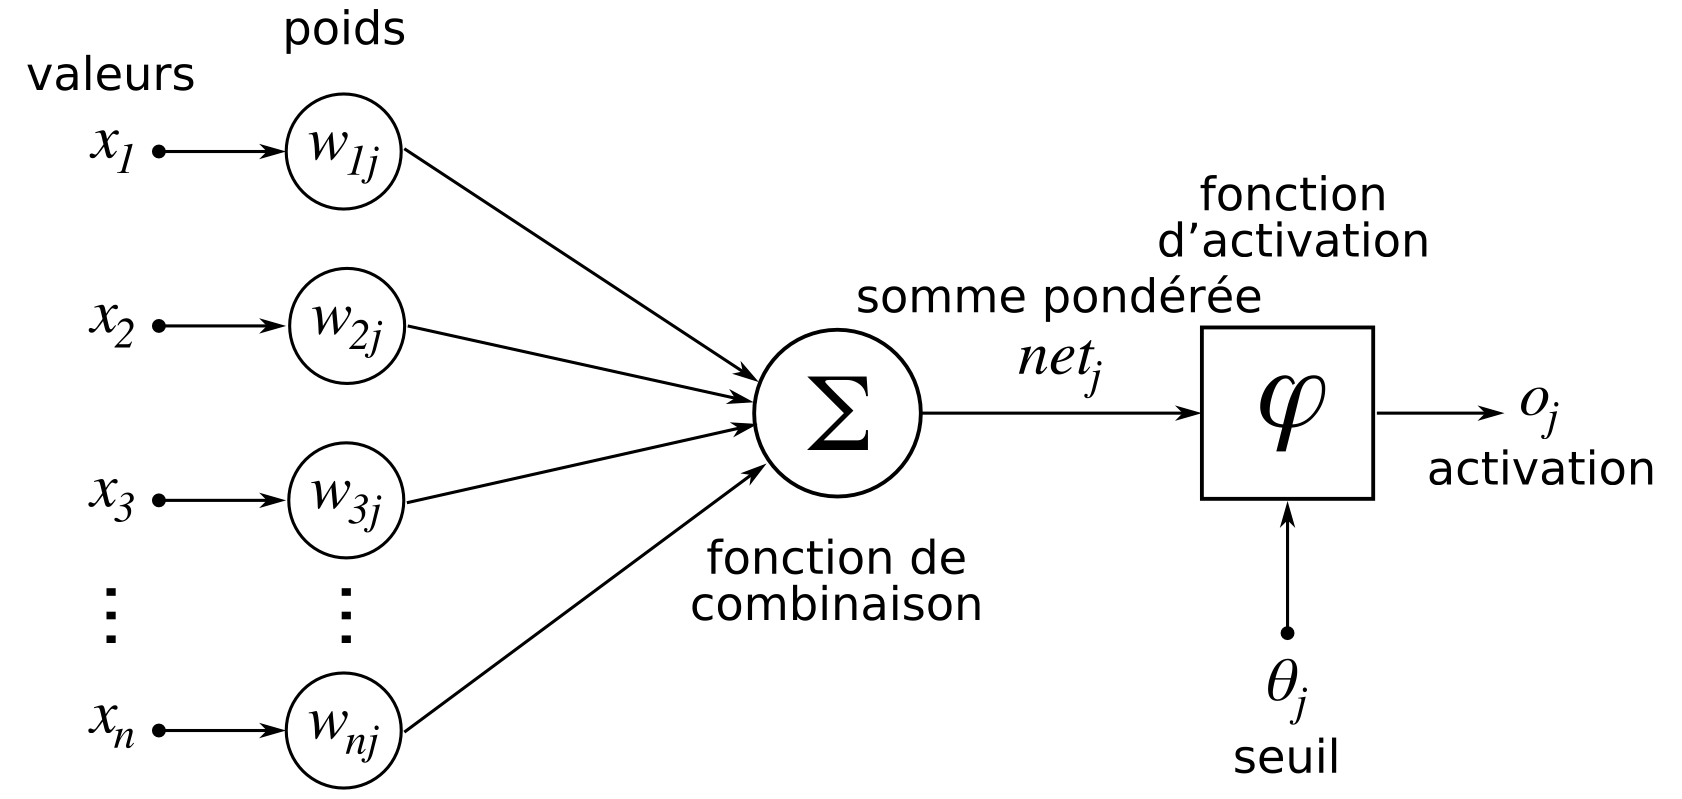
\includegraphics[width=0.6\textwidth]{img/ltu.png}
\caption{Unité Linéaire à Seuil}
\label{fig:ltu}
\end{figure}

Après avoir calculé une combinaison linéaire des entrées, il applique une fonction seuil. Sa sortie vaut :
\[o = \phi(\langle \boldsymbol{w}, \boldsymbol{x} \rangle)\]
où : \(\phi\) est la fonction seuil; \(\boldsymbol{w}\) est le vecteur des \(n\) poids associés aux entrées; \(\boldsymbol{x}\) est le vecteur des \(n\) entrées.

Un LTU a son utilité dans une classification binaire lorsqu'il est utilisé seul, ou dans une classification multiple lorsqu'il est combiné à d'autres LTU. Cependant, tel quel, il est incapable de séparer des points autrement que par une frontière linéaire. Par exemple, simplement pour mimer le comportement de la fonction OU EXCLUSIF (XOR), il faut plusieurs LTU pour séparer les points identiques.

\begin{figure}[H]
\centering
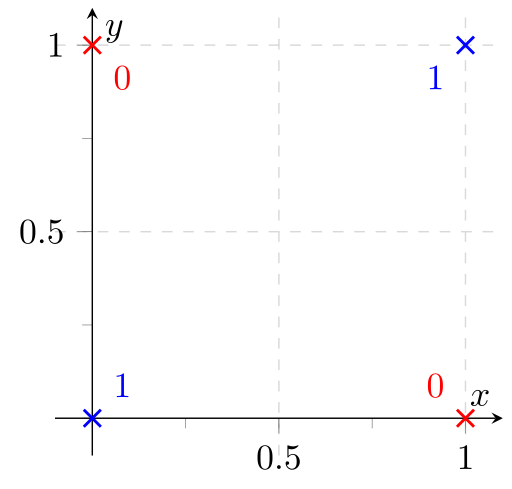
\includegraphics[width=0.4\textwidth]{img/xor.png}
\caption{Fonction XOR\((x,y)\)}
\label{fig:xor}
\end{figure}

Puisque les points de la fonction XOR ne sont pas linéairement séparables, il n'est pas étonnant qu'un seul LTU ne s'en sorte pas. Mais l'apparente faiblesse des LTU face à un problème si simple a quelque peu déçu les chercheurs des années 50-60, qui ont alors pu abandonner le connexionisme. Mais nous verrons que les LTU seuls ou en réseau sont loin d'être inutiles. 

Voyons maintenant quelles modifications ont été apportées depuis.

\subsection{Neurone non linéaire}
Un désavantage majeur des LTU est que leur sortie, binaire, est calculée par une fonction seuil. Ceci mène à une frontière de séparation linéaire dans l'espace des variables d'entrée. Bien que la simplicité des modèles linéaires ait fait ses preuves par le passé, il est parfois nécessaire de complexifier. Ainsi, une modification envisagée fut de remplacer la fonction seuil par une des fonctions suivantes (ou par une des nombreuses autres existantes) : 
\begin{align}
\sigma &: t \mapsto \frac{1}{1 + e^{-t}}\\
\tanh &: t \mapsto \frac{e^t - e^{-t}}{e^t + e^{-t}}\\
\mathit{ReLU} &: t \mapsto max(0, t)
\end{align}

Elles sont représentées graphiquement autour de \((0, 0)\) par la figure \ref{fig:activations}. 

\begin{figure}[H]
\centering
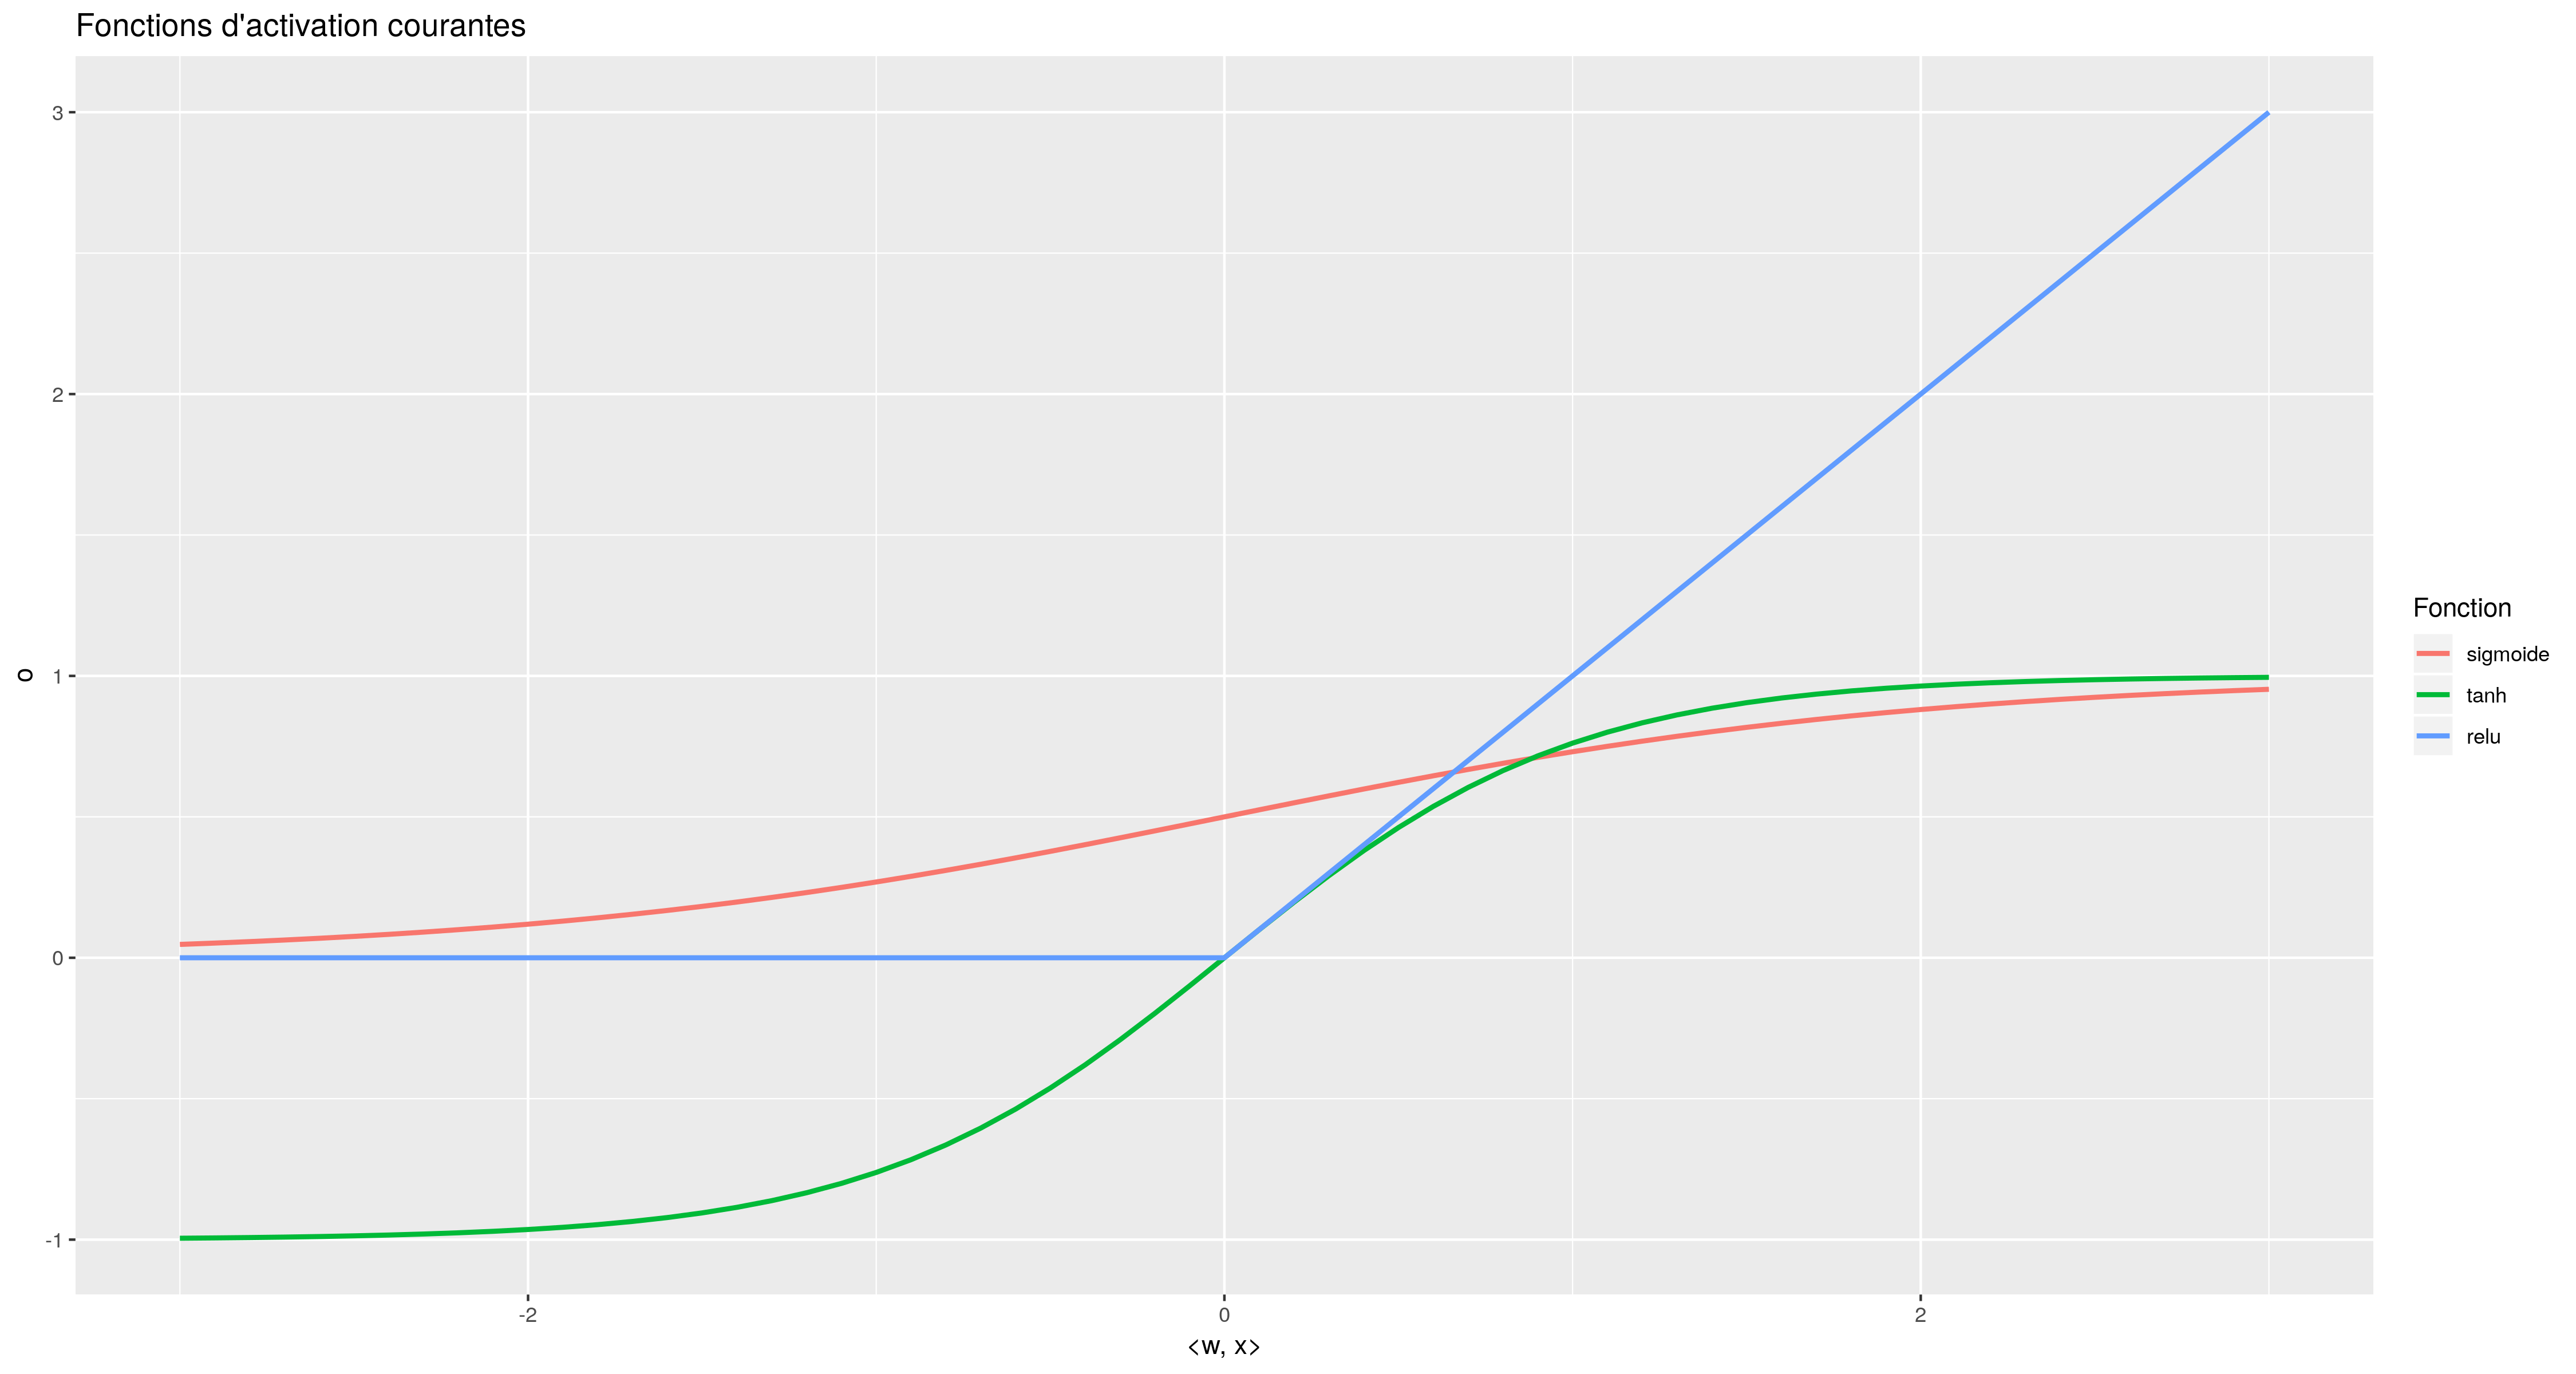
\includegraphics[width=\textwidth]{img/activations.png}
\caption{Les fonctions d'activation citées}
\label{fig:activations}
\end{figure}

Un autre ajout fut celui d'un terme constant, appelé \emph{biais} avant la \emph{fonction d'activation}. En conservant les mêmes notations que précédemment, l'équation en sortie du neurone est donc la suivante : 
\begin{equation}\label{eq:neurone}
o = \phi(\langle \boldsymbol{w}, \boldsymbol{x} \rangle + b)
\end{equation}

Le biais du neurone sert à activer celui-ci même lorsque le signal d'entrée est faible. Dans un réseau, cela aura pour effet de déclencher l'apprentissage chez au moins quelques neurones.

L'intérêt des neurones non linéaires apparaît vraiment lorsqu'on les regroupe en réseaux.

\section{Réseaux de neurones}
Voici un aperçu de ce à quoi un réseaux de neurones peut ressembler :

\begin{figure}[H]
\centering
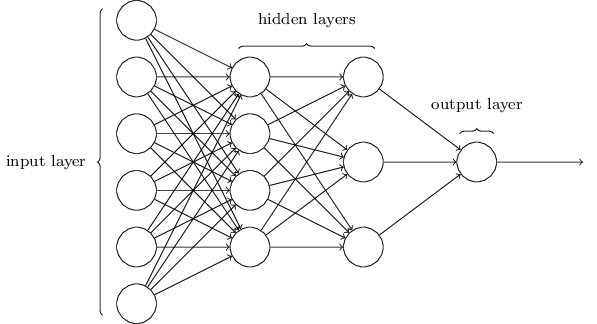
\includegraphics[width=0.8\textwidth]{img/reseau_neurones.png}
\caption{Un exemple de réseau de neurones}
\label{fig:ffnn}
\end{figure}

On y voit une \emph{couche d'entrée} (\emph{input layer}), des \emph{couches cachées} (\emph{hidden layers}) et une \emph{couche de sortie} (\emph{output layer}). Mais, contrairement au neurone seul, on ne peut pas simplement expliciter la sortie du réseau en fonction des entrées. Nous expliquerons en détail aux chapitres suivants comment travailler avec de tels réseaux.


\section{Dilemme biais - variance, ajustement}
Imaginons la situation suivante: deux amis, Béatrice et Valentin, se baladent et croisent un artiste de rue. Celui-ci leur présente une pièce de monnaie et les assure qu'elle n'est pas truquée. Sans tarder, il leur propose de deviner de quel côté tombera la pièce au 9e lancer,  après avoir regardé les 8 premiers lancers. Les deux amis constatent qu'à chacun des 8 lancers, la pièce est tombée sur pile, mais interprètent les résultats différemment. Pour Béatrice, chaque lancer est indépendant du précédent, et on leur a de plus dit que la pièce n'était pas truquée; elle en conclut que les deux faces sont équiprobables au 9e lancer. Valentin n'est pas d'accord. Selon lui, on ne peut pas faire confiance à ce qu'a dit l'artiste de rue au début, les données "parlent" d'elles-mêmes; il en conclut que la pièce tombera sur pile.

Malheureusement, l'histoire ne dit précise pas la suite des évènements, on peut malgré tout en tirer des leçons. Le raisonnement de Valentin souffre d'un défaut relativement facile à déceler, appelé \emph{sur-ajustement} (on parle aussi de \emph{sur-interprétation} ou de \emph{sur-apprentissage}, \emph{overfitting} en anglais), qui survient lorsqu'on cherche à généraliser des données mais à partir d'un modèle qui les ajuste parfaitement. En résumé, Valentin a tendance à trop "coller" aux données, en leur faisant aveuglément confiance. Dans ce cas précis, on pressent qu'il tend à surajuster car, sous l'hypothèse que la pièce est équilibrée, 8 tirages identiques d'affilée surviennent tous les 256 lancer environ. Ainsi, Valentin n'a pas suffisamment de données pour écarter si drastiquement le modèle de Béatrice. En revanche, si nos deux amis avaient été témoins de plus de lancers identiques, disons 50, il aurait été bien plus légitime de conclure que le modèle d'équiprobabilité est faux.

Malgré tout, son amie n'a pas tout à fait raison non plus. L'approche de Béatrice se fonde sur un modèle très simplifié de la réalité, et les prémisses de celui-ci peuvent être fausses. Dans le cas d'une pièce de monnaie, il est possible de s'entraîner à la lancer et la rattraper de sorte à en contrôler l'issue avec une forte probabilité. Des études spécifiques on été menées sur des pièces de 1 euro et 2 euros, concluant qu'elles n'étaient pas équilibrées\footnote{\url{https://www.youtube.com/watch?v=AYnJv68T3MM}}. Dans le cas de Béatrice, lorsqu'on fait trop confiance à un modèle et pas assez aux données, on parle de \emph{sous-ajustement} (\emph{sous-apprentissage}, ou encore de \emph{sous-interprétation} , \emph{underfitting} en anglais).

Cet exemple élémentaire sert à illustrer un problème central de l'apprentissage artificiel: le dilemme entre diminuer le biais\footnote{Ce biais, notion statistique, n'a rien à voir avec celui des neurones artificiels.} et diminuer la variance. Un résultat important en statistiques et apprentissage artificiel est que l'erreur de généralisation d'un modèle  possède trois sources d'erreur différentes : 
\begin{description}
\item [Biais] Il est dû à des mauvaises hypothèses, comme par exemple considérer que des données obéissent à un modèle linéaire alors qu'un processus quadratique en est réellement à l'origine. Un modèle à haut biais a tendance à sous-ajuster les données.
\item [Variance] Elle résulte d'une sensibilité excessive du modèle vis-à-vis des données. C'est typiquement le cas des modèles de régression polynomiaux à degré élevé. Un modèle à haute variance a tendance à sur-ajuster les données.
\item[Erreur résiduelle] Cette dernière forme d'erreur est ce qu'on appelle parfois le "bruit" qui s'immisce dans les données. L'unique moyen de s'en débarrasser est de réparer les sources de données, comme des capteurs défaillants par exemple, ou d'ignorer les données aberrantes. Cette tâche est loin d'être aisée dans le cas général.
\end{description}

Tenter de réduire le biais d'un modèle revient à en augmenter la variance, et vice versa, d'où le terme de "dilemme" ou "compromis" biais-variance.

Nous décrirons plus loin comment déceler la sur-interprétation et la sous-interprétation, ainsi que diverses techniques pour les éviter.

\section{Protocole pour un problème d'apprentissage}
Une partie importante du travail est faite lors de l'analyse du problème à résoudre. Voici une approche assez générale pour clarifier les points précédents :

\begin{description}
\item [Données à traiter] Est-ce du texte, des images, du son, de la vidéo ?
\item [Format des données] S'agit-il des fichiers colonnes à en-têtes, du texte brut, des images (éventuellement compressées), du son très riche ?
\item [Sortie de l'algorithme] L'algorithme doit-il prédire un mot, une phrase, une valeur numérique, une couleur, une image ?
\item [Structures des observations] Les observations sont-elles distribuées de manière normale, bimodale, par petits groupes, sur une droite, sur un hyperplan ? 
\item [Modèle adapté] L'état de l'art suggère-t-il une régression linéaire, une régression polynomiale, un classifieur linéaire, un réseau de neurones ?
\end{description}

Ne pas répondre (correctement) à ces questions avant de se lancer dans la programmation est une erreur souvent fatale.

\section{Conclusion}
Nous avons ici succinctement présenté quelques manières de catégoriser les solutions à un problème d'apprentissage automatique, de la régression linéaire à l'apprentissage non supervisé et aux réseaux de neurones profonds. Enfin, nous avons vu un rapide protocole nous permettant de décider quelle solution envisager d'abord lorsqu'on doit résoudre un problème d'apprentissage ou d'intelligence artificielle.

Malheureusement, il n'est pas possible de rédiger un état de l'art des techniques et des technologies de ce domaine sans écrire un (très gros) livre. Cependant, survoler les méthodes tout en mettant l'accent sur les principes reste intéressant.

Nous verrons, au prochain chapitre, comment entraîner et évaluer un réseau de neurones, et les problématiques qui émergent lorsque la taille du réseau augmente.